\chapter{Introduction}\label{cha:intro}
Discrepancies in measurements of the rotations of galaxies indicate the presence of a large amount of matter which interacts through gravity, though not electromagnetically making it invisible. This matter is commonly referred to as dark matter. Since no known or hypothesised particle in the standard model of particle physics can be used as a candidate for dark matter, this has opened the door for new physics. Aside form this there are other phenomena that can not be explained today. One of the proposed models to correct these discrepancies is known as Supersymmetry (SUSY).  


In this chapter an introduction to both the theoretical and experimental details are given. 
Explain the phase 2 high luminosity upgrade? Or atleast refer to where more is written.
Why was this topic chosen? What is the purpose of the introduction?

\newpage
\section{Research goal}\label{sec:goal}
This research took place at Stockholm University from January 7th until \textbf{when?}
During the research period the following tasks were set up and performed/answered:
\begin{itemize}
\item Implement a C++ programme that loops over the collisions inside the signal and background datasets.	
\item For each collision retrieve the relevant observables (variables used to	 extract the signal over the background) and apply "smearing functions" to emulate the effect of the high luminosity on the observables. 	
\item For both signal and background datasets, compare observables before and after smearing. What observables are the least/most affected?	
\item Implement selection criteria that selects the signal collisions efficiently while reduces significantly the background. In a first step the selection criteria should be taken from existing studies.
\item Selection criteria can be evaluated and compared with each other using a figure of merit Z, that measures the sensitivity of the experiment to the	 dark matter signal. Calculate Z for the given selection criteria before and after smearing.
\item What is the effect of the high luminosity (smearing) on the value of Z?
\item Investigate other selection criteria and observables, to mitigate the effect of high luminosity. Use Z to rank different criteria after smearing.
\item Conclude on the effect of the high luminosity on the sensitivity for dark matter and possible ways to mitigate its effects using alternative observables and selection criteria. 
\end{itemize}
\newpage
\section{Theoretical Background}\label{sec:tb}
The following is a short description of the theory which is required to understand this thesis. Find more information in (references).
\subsection{Quantum mechanics and quantum field theory}
Speak about: Why QM, Lagrangian refer to classical mechanics, end with hand of to particle physics. need to explain observables.

Dont forget to explain cross-sections from qft.
\subsection{Four-vectors}
\subsection{Effective field theory}
Which one do we use? What parameters have we joined?
How does this pertain to the rest?

\subsection{Nuclear, particle and subatomic particle physics}
Can be seen as the experimental counterpart to quantum mechanics.
Many could argue that these branches started after Ernest Rutherford famous gold foil experiment (reference), where he discovered that matter is composed of matter with a nucleus, a lot of empty space and electrons. This and more sparked the curiosity to see what the nucleus was made of and so on... 

The discovery of the quark diving of bosons/fermions different generations. Fundamental particles. Basically all of 20th century physics. 

Some thing so that a description of particles are in here, end with standard model.
Content should be enough for the rest of the thesis regarding collisions etc.
Luminosity!

\subsection{The standard model of particle physics} 
How and why is there a standard model? give the Lagrangian and refer to all the different interactions that are included. Which then combines QM with subatomic particle physics.
 
Mention Antimatter!
Is it proved? What problems exist? 

\subsection{Beyond the standard model: Supersymmetry}
In the early 1970:s similar as QED expansion with antimatter due to (integral which one diverged?). Similarly to this, an expansion with a similar symmetry having bosons instead of fermions and the reverse. These symmetrical particles are known as supersymmetrical partners. The SUSY partner of a boson is denoted as sfermion (squarks and sleptons) whereas the SUSY partner of a fermion is denoted as bosinos (gauginos)

Different problems, hierarchy, etc

Bring up different expansions. Here we will talk about supersymmetry (SUSY) end with neutrilino/WIMPS. 
Minimal Supersymmetric Standard Model

Supersymmetry: Every boson has a supersymmetrical fermion, and the reverse.
\subsection{Dark matter: Concept}
\subsection{Dark matter: Candidates}
Weakly interacting massive particles (Wimps) are a candidate to explain Dark matter, it is this candidate which is considered in this thesis.
In addition the condition that the WIMPS are Dirac fermions (fermions which are not their own antiparticle) is implied.

In \ref{tab:operators} the operators which are integrated out via the effective field theory and are of interest itn theis thesis are given.
\renewcommand{\arraystretch}{1.5} %Change height of tabel
\begin{table}[H]
\begin{center}
    \begin{tabular}{ | l | l | l | l |}
    \hline
    Name & Initial state & Type & Operator \\ \hline
  	D1 & qq & scalar & $\frac{m_q}{M^3_*} \bar{\chi} \chi \bar{q} q$ \\ \hline
  	D5 & qq & vector & $\frac{1}{M^2_*} \bar{\chi} \gamma^\mu \chi \bar{q} \gamma_\mu q$ \\ \hline
  	D8 & qq & axial-vector & $\frac{1}{M^2_*}\bar{\chi}\gamma^\mu \gamma^5 \chi \bar{q} \gamma_\mu \gamma^5 q $ \\ \hline
  	D9 & qq & tensor & $\frac{1}{M^2_*} \bar{\chi}\sigma^{\mu \nu} \chi \bar{q} \sigma_{\mu \nu} q  $\\ \hline
  	D11 & gg & scalar & $\frac{1}{4M^3_*}\bar{\chi}\chi \alpha_s (G^a_{\mu \nu})^2 $\\ \hline
  	\end{tabular}

  	\caption{From \citep{CERN-PH-EP-2012-210}}
  	\label{tab:operators}
  	  	\end{center}
    \end{table}
\renewcommand{\arraystretch}{1.0}  %Back to default
Where D denotes that the WIMPS are assumed to be Dirac fermions.

Alot here taken from \citep{82.116010}

\subsection{Search for WIMPS}
Since the search for WIMPS at the LHC is based on looking at $E_T^{Miss}$ it will be canonical though the experiment can no establish if a WIMP is stable on a cosmological time scale and thus if it is a Dark matter candidate \citep{CERN-PH-EP-2012-210}


What is it? Why at CERN/ATLAS? Candidates?
Dark matter is something which does not interact electromagnetically however it does have a gravitational effect on nearby bodies.
Cold dark matter?
Non-barionic dark matter. Why not barionic?
WIMPS, wimps as candidates.
How is this detectable at ATLAS? Finish with this. Refer next chapter and that neutralinos are a candidate.

\newpage
\section{Experimental overview}
What was used in this research and what needs to be explained? Upgrade, pileup etc.
Somewhere here explain how the radial coordinate system is defined.
\subsection{Cern}
\subsection{LHC}
\subsection{ATLAS}
\subsection{Coordinate system}
Something something

\begin{figure}[H]
\begin{center}
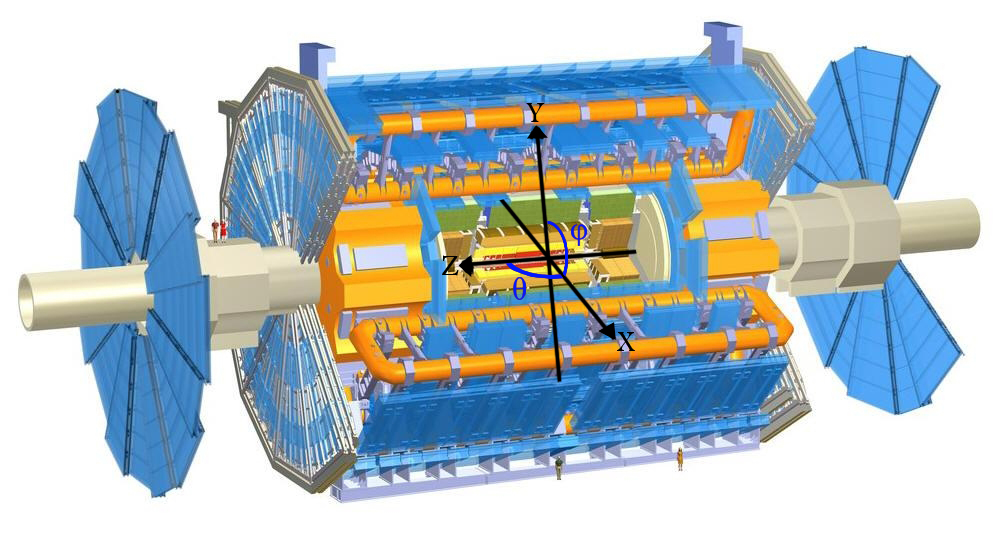
\includegraphics[scale=0.25]{particle_collider.jpg}
\label{fig:coordinatesystem}
\caption{Figure showing the ATLAS detector and the definition of the coordinate system. Image altered from original taken from\citep{coordimage}}
\end{center}
\end{figure}



\subsection{Commonly used four-vectors}
\subsection{Calorimeter}
\subsection{Truth and reconstructed data}
Give a general description.

In this thesis, truth = Montecarlo. 
Reconstructed data = that which is seen in the detectors, which is the smeared data.
\subsection{Jet and missing energy}
What is a jet? why are we only looking at transverse missing energy? 

\subsection{Phase II high luminosity upgrade}
I am looking at the upgrade which will be done at CERN and will be completed around 2022-2023 and is denoted High Luminosity-LHC Phase 2 upgrade. When this is running the following is expected:
\begin{table}[H]
\begin{center}
    \begin{tabular}{ | l | l | l |}
    \hline
    Entity & Expected & Last run (2012) \\ \hline
  	Luminosity & 1000-3000 $fb^{-1}$ & 20.8 $fb^{-1}$ \\ \hline
  	Pile-up & $\obs{\mu}=200$ & $\obs{\mu}=20.7$ \\ \hline
  	Center of mass energy & $\sqrt{s}=14$ TeV &  $\sqrt{s}=8$ TeV \\ \hline
  	\end{tabular}
  	
  	\caption{Expected running values for the Phase II HL-upgraded LHC with older values for comparison. REFERENCE?}
  	\label{tab:expectvalues}
  	\end{center}
    \end{table}
Taken from "a short explanation of different terminology by me" Find a cern source.
Assumed effects, timespan when will it be done?
